\documentclass[twoside]{book}

% Packages required by doxygen
\usepackage{fixltx2e}
\usepackage{calc}
\usepackage{doxygen}
\usepackage[export]{adjustbox} % also loads graphicx
\usepackage{graphicx}
\usepackage[utf8]{inputenc}
\usepackage{makeidx}
\usepackage{multicol}
\usepackage{multirow}
\PassOptionsToPackage{warn}{textcomp}
\usepackage{textcomp}
\usepackage[nointegrals]{wasysym}
\usepackage[table]{xcolor}

% Font selection
\usepackage[T1]{fontenc}
\usepackage[scaled=.90]{helvet}
\usepackage{courier}
\usepackage{amssymb}
\usepackage{sectsty}
\renewcommand{\familydefault}{\sfdefault}
\allsectionsfont{%
  \fontseries{bc}\selectfont%
  \color{darkgray}%
}
\renewcommand{\DoxyLabelFont}{%
  \fontseries{bc}\selectfont%
  \color{darkgray}%
}
\newcommand{\+}{\discretionary{\mbox{\scriptsize$\hookleftarrow$}}{}{}}

% Page & text layout
\usepackage{geometry}
\geometry{%
  a4paper,%
  top=2.5cm,%
  bottom=2.5cm,%
  left=2.5cm,%
  right=2.5cm%
}
\tolerance=750
\hfuzz=15pt
\hbadness=750
\setlength{\emergencystretch}{15pt}
\setlength{\parindent}{0cm}
\setlength{\parskip}{3ex plus 2ex minus 2ex}
\makeatletter
\renewcommand{\paragraph}{%
  \@startsection{paragraph}{4}{0ex}{-1.0ex}{1.0ex}{%
    \normalfont\normalsize\bfseries\SS@parafont%
  }%
}
\renewcommand{\subparagraph}{%
  \@startsection{subparagraph}{5}{0ex}{-1.0ex}{1.0ex}{%
    \normalfont\normalsize\bfseries\SS@subparafont%
  }%
}
\makeatother

% Headers & footers
\usepackage{fancyhdr}
\pagestyle{fancyplain}
\fancyhead[LE]{\fancyplain{}{\bfseries\thepage}}
\fancyhead[CE]{\fancyplain{}{}}
\fancyhead[RE]{\fancyplain{}{\bfseries\leftmark}}
\fancyhead[LO]{\fancyplain{}{\bfseries\rightmark}}
\fancyhead[CO]{\fancyplain{}{}}
\fancyhead[RO]{\fancyplain{}{\bfseries\thepage}}
\fancyfoot[LE]{\fancyplain{}{}}
\fancyfoot[CE]{\fancyplain{}{}}
\fancyfoot[RE]{\fancyplain{}{\bfseries\scriptsize Generated by Doxygen }}
\fancyfoot[LO]{\fancyplain{}{\bfseries\scriptsize Generated by Doxygen }}
\fancyfoot[CO]{\fancyplain{}{}}
\fancyfoot[RO]{\fancyplain{}{}}
\renewcommand{\footrulewidth}{0.4pt}
\renewcommand{\chaptermark}[1]{%
  \markboth{#1}{}%
}
\renewcommand{\sectionmark}[1]{%
  \markright{\thesection\ #1}%
}

% Indices & bibliography
\usepackage{natbib}
\usepackage[titles]{tocloft}
\setcounter{tocdepth}{3}
\setcounter{secnumdepth}{5}
\makeindex

% Hyperlinks (required, but should be loaded last)
\usepackage{ifpdf}
\ifpdf
  \usepackage[pdftex,pagebackref=true]{hyperref}
\else
  \usepackage[ps2pdf,pagebackref=true]{hyperref}
\fi
\hypersetup{%
  colorlinks=true,%
  linkcolor=blue,%
  citecolor=blue,%
  unicode%
}

% Custom commands
\newcommand{\clearemptydoublepage}{%
  \newpage{\pagestyle{empty}\cleardoublepage}%
}

\usepackage{caption}
\captionsetup{labelsep=space,justification=centering,font={bf},singlelinecheck=off,skip=4pt,position=top}

%===== C O N T E N T S =====

\begin{document}

% Titlepage & ToC
\hypersetup{pageanchor=false,
             bookmarksnumbered=true,
             pdfencoding=unicode
            }
\pagenumbering{roman}
\begin{titlepage}
\vspace*{7cm}
\begin{center}%
{\Large My Project }\\
\vspace*{1cm}
{\large Generated by Doxygen 1.8.11}\\
\end{center}
\end{titlepage}
\clearemptydoublepage
\tableofcontents
\clearemptydoublepage
\pagenumbering{arabic}
\hypersetup{pageanchor=true}

%--- Begin generated contents ---
\chapter{Hierarchical Index}
\section{Class Hierarchy}
This inheritance list is sorted roughly, but not completely, alphabetically\+:\begin{DoxyCompactList}
\item Move\+Group\+Commander\begin{DoxyCompactList}
\item \contentsline{section}{ms\+Move\+Group.\+ms\+Move\+Group}{\pageref{classmsMoveGroup_1_1msMoveGroup}}{}
\item \contentsline{section}{ms\+Move\+Group\+Old.\+ms\+Move\+Group}{\pageref{classmsMoveGroupOld_1_1msMoveGroup}}{}
\end{DoxyCompactList}
\item \contentsline{section}{ms\+Math.\+online\+Standard\+Deviations}{\pageref{classmsMath_1_1onlineStandardDeviations}}{}
\item \contentsline{section}{ms\+Tf\+Getter.\+tf\+Getter}{\pageref{classmsTfGetter_1_1tfGetter}}{}
\end{DoxyCompactList}

\chapter{Class Index}
\section{Class List}
Here are the classes, structs, unions and interfaces with brief descriptions\+:\begin{DoxyCompactList}
\item\contentsline{section}{\hyperlink{classkondoServoLib_1_1b3mCtrl_07_xE3_x82_xB3_xE3_x83_x94_xE3_x83_xBC_08_1_1B3mClass}{kondo\+Servo\+Lib.\+b3m\+Ctrl(コピー).\+B3m\+Class} }{\pageref{classkondoServoLib_1_1b3mCtrl_07_xE3_x82_xB3_xE3_x83_x94_xE3_x83_xBC_08_1_1B3mClass}}{}
\item\contentsline{section}{\hyperlink{classkondoServoLib_1_1b3mCtrl_1_1B3mClass}{kondo\+Servo\+Lib.\+b3m\+Ctrl.\+B3m\+Class} }{\pageref{classkondoServoLib_1_1b3mCtrl_1_1B3mClass}}{}
\item\contentsline{section}{\hyperlink{classkondoServoLib_1_1ctrlKondoServo_1_1ctrlKondoServoClass}{kondo\+Servo\+Lib.\+ctrl\+Kondo\+Servo.\+ctrl\+Kondo\+Servo\+Class} }{\pageref{classkondoServoLib_1_1ctrlKondoServo_1_1ctrlKondoServoClass}}{}
\item\contentsline{section}{\hyperlink{classkondoServoLib_1_1icsCtrl_1_1IcsClass}{kondo\+Servo\+Lib.\+ics\+Ctrl.\+Ics\+Class} }{\pageref{classkondoServoLib_1_1icsCtrl_1_1IcsClass}}{}
\end{DoxyCompactList}

\chapter{Class Documentation}
\hypertarget{classkondoServoLib_1_1b3mCtrl_07_xE3_x82_xB3_xE3_x83_x94_xE3_x83_xBC_08_1_1B3mClass}{}\section{kondo\+Servo\+Lib.\+b3m\+Ctrl(コピー).B3m\+Class Class Reference}
\label{classkondoServoLib_1_1b3mCtrl_07_xE3_x82_xB3_xE3_x83_x94_xE3_x83_xBC_08_1_1B3mClass}\index{kondo\+Servo\+Lib.\+b3m\+Ctrl(コピー).\+B3m\+Class@{kondo\+Servo\+Lib.\+b3m\+Ctrl(コピー).\+B3m\+Class}}


Inheritance diagram for kondo\+Servo\+Lib.\+b3m\+Ctrl(コピー).B3m\+Class\+:\nopagebreak
\begin{figure}[H]
\begin{center}
\leavevmode
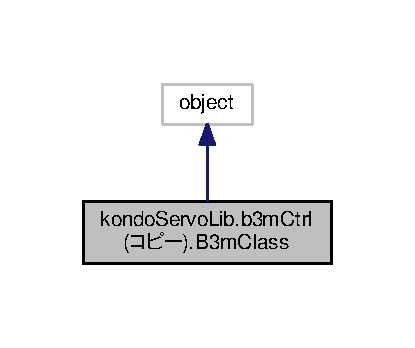
\includegraphics[width=199pt]{classkondoServoLib_1_1b3mCtrl_07_xE3_x82_xB3_xE3_x83_x94_xE3_x83_xBC_08_1_1B3mClass__inherit__graph}
\end{center}
\end{figure}


Collaboration diagram for kondo\+Servo\+Lib.\+b3m\+Ctrl(コピー).B3m\+Class\+:\nopagebreak
\begin{figure}[H]
\begin{center}
\leavevmode
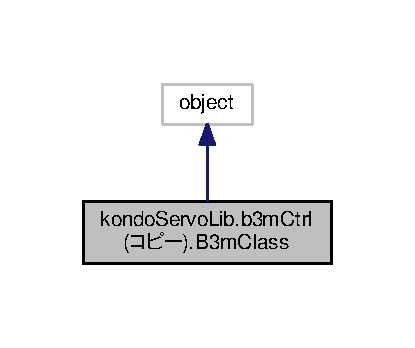
\includegraphics[width=199pt]{classkondoServoLib_1_1b3mCtrl_07_xE3_x82_xB3_xE3_x83_x94_xE3_x83_xBC_08_1_1B3mClass__coll__graph}
\end{center}
\end{figure}
\subsection*{Public Member Functions}
\begin{DoxyCompactItemize}
\item 
def {\bfseries \+\_\+\+\_\+init\+\_\+\+\_\+} (self, \+\_\+port=None, \+\_\+baudrate=1500000, \+\_\+timeout=0.\+005)\hypertarget{classkondoServoLib_1_1b3mCtrl_07_xE3_x82_xB3_xE3_x83_x94_xE3_x83_xBC_08_1_1B3mClass_aeed52d02373a5dc57b5a55e4ea1fc789}{}\label{classkondoServoLib_1_1b3mCtrl_07_xE3_x82_xB3_xE3_x83_x94_xE3_x83_xBC_08_1_1B3mClass_aeed52d02373a5dc57b5a55e4ea1fc789}

\item 
def {\bfseries \+\_\+\+\_\+del\+\_\+\+\_\+} (self)\hypertarget{classkondoServoLib_1_1b3mCtrl_07_xE3_x82_xB3_xE3_x83_x94_xE3_x83_xBC_08_1_1B3mClass_a770de49ce6347a36a406b5ebbb28999b}{}\label{classkondoServoLib_1_1b3mCtrl_07_xE3_x82_xB3_xE3_x83_x94_xE3_x83_xBC_08_1_1B3mClass_a770de49ce6347a36a406b5ebbb28999b}

\item 
def \hyperlink{classkondoServoLib_1_1b3mCtrl_07_xE3_x82_xB3_xE3_x83_x94_xE3_x83_xBC_08_1_1B3mClass_a1252a9de80537da4ea39d8b79e595f4f}{begin} (self, \+\_\+port=None, \+\_\+baudrate=None, \+\_\+timeout=None)
\begin{DoxyCompactList}\small\item\em 通信開始設定 \end{DoxyCompactList}\item 
def \hyperlink{classkondoServoLib_1_1b3mCtrl_07_xE3_x82_xB3_xE3_x83_x94_xE3_x83_xBC_08_1_1B3mClass_afdadbab52ffc1bfd82b400f8df29a54f}{load\+Cmd} (self, id, option=\char`\"{}E\+R\+R\+OR\char`\"{})
\begin{DoxyCompactList}\small\item\em R\+O\+Mを\+R\+A\+Mに書き込み(シングル/マルチ) \end{DoxyCompactList}\item 
def \hyperlink{classkondoServoLib_1_1b3mCtrl_07_xE3_x82_xB3_xE3_x83_x94_xE3_x83_xBC_08_1_1B3mClass_a6b1853c66d7addd2090823c3a3837792}{save\+Cmd} (self, id, option=\char`\"{}E\+R\+R\+OR\char`\"{})
\begin{DoxyCompactList}\small\item\em R\+A\+Mを\+R\+O\+Mに書き込み(シングル/マルチ) \end{DoxyCompactList}\item 
def \hyperlink{classkondoServoLib_1_1b3mCtrl_07_xE3_x82_xB3_xE3_x83_x94_xE3_x83_xBC_08_1_1B3mClass_a99f249f885c3b4765383e67666720160}{read\+Cmd} (self, id, address, length, option=\char`\"{}E\+R\+R\+OR\char`\"{})
\begin{DoxyCompactList}\small\item\em R\+A\+Mの読み出し(シングル) \end{DoxyCompactList}\item 
def \hyperlink{classkondoServoLib_1_1b3mCtrl_07_xE3_x82_xB3_xE3_x83_x94_xE3_x83_xBC_08_1_1B3mClass_ab105d7d42e31d00370ebe043057a98ec}{write\+Cmd} (self, id, address, data, option=\char`\"{}E\+R\+R\+OR\char`\"{})
\begin{DoxyCompactList}\small\item\em R\+A\+Mへの書き込み(シングル/マルチ) \end{DoxyCompactList}\item 
def \hyperlink{classkondoServoLib_1_1b3mCtrl_07_xE3_x82_xB3_xE3_x83_x94_xE3_x83_xBC_08_1_1B3mClass_a559506a0d8f00a75ac724d99c8849707}{reset\+Cmd} (self, id, time=0, option=\char`\"{}E\+R\+R\+OR\char`\"{})
\begin{DoxyCompactList}\small\item\em 再起動要求(シングル/マルチ) \end{DoxyCompactList}\item 
def \hyperlink{classkondoServoLib_1_1b3mCtrl_07_xE3_x82_xB3_xE3_x83_x94_xE3_x83_xBC_08_1_1B3mClass_aa359b291efcd618e32c411e3d070ff76}{position\+Cmd} (self, id, pos, time=0, option=\char`\"{}E\+R\+R\+OR\char`\"{})
\begin{DoxyCompactList}\small\item\em 位置設定(シングル/マルチ) \end{DoxyCompactList}\item 
def {\bfseries set\+Mode} (self, id, mode, option=\char`\"{}E\+R\+R\+OR\char`\"{})\hypertarget{classkondoServoLib_1_1b3mCtrl_07_xE3_x82_xB3_xE3_x83_x94_xE3_x83_xBC_08_1_1B3mClass_a37b99b97aebc68b1df4f2d6d28ecf004}{}\label{classkondoServoLib_1_1b3mCtrl_07_xE3_x82_xB3_xE3_x83_x94_xE3_x83_xBC_08_1_1B3mClass_a37b99b97aebc68b1df4f2d6d28ecf004}

\item 
def {\bfseries set\+Trajectory\+Type} (self, id, \+\_\+type, option=\char`\"{}E\+R\+R\+OR\char`\"{})\hypertarget{classkondoServoLib_1_1b3mCtrl_07_xE3_x82_xB3_xE3_x83_x94_xE3_x83_xBC_08_1_1B3mClass_aa53b678be54acc242cc5f8e19bd4d84f}{}\label{classkondoServoLib_1_1b3mCtrl_07_xE3_x82_xB3_xE3_x83_x94_xE3_x83_xBC_08_1_1B3mClass_aa53b678be54acc242cc5f8e19bd4d84f}

\item 
def {\bfseries set\+Ram} (self, id, data, property, option=\char`\"{}E\+R\+R\+OR\char`\"{})\hypertarget{classkondoServoLib_1_1b3mCtrl_07_xE3_x82_xB3_xE3_x83_x94_xE3_x83_xBC_08_1_1B3mClass_a5a9f824f9df9aadd869fc6c9a396e4e9}{}\label{classkondoServoLib_1_1b3mCtrl_07_xE3_x82_xB3_xE3_x83_x94_xE3_x83_xBC_08_1_1B3mClass_a5a9f824f9df9aadd869fc6c9a396e4e9}

\item 
def {\bfseries get\+Ram} (self, id, property, option=\char`\"{}E\+R\+R\+OR\char`\"{})\hypertarget{classkondoServoLib_1_1b3mCtrl_07_xE3_x82_xB3_xE3_x83_x94_xE3_x83_xBC_08_1_1B3mClass_a5c8454698cc2e635d0615a8fdbc6e119}{}\label{classkondoServoLib_1_1b3mCtrl_07_xE3_x82_xB3_xE3_x83_x94_xE3_x83_xBC_08_1_1B3mClass_a5c8454698cc2e635d0615a8fdbc6e119}

\item 
def {\bfseries set\+New\+Id} (self, current\+Id, new\+Id)\hypertarget{classkondoServoLib_1_1b3mCtrl_07_xE3_x82_xB3_xE3_x83_x94_xE3_x83_xBC_08_1_1B3mClass_afbe75567bbd0b9f3412c02acc2a2c1dd}{}\label{classkondoServoLib_1_1b3mCtrl_07_xE3_x82_xB3_xE3_x83_x94_xE3_x83_xBC_08_1_1B3mClass_afbe75567bbd0b9f3412c02acc2a2c1dd}

\end{DoxyCompactItemize}
\subsection*{Static Public Member Functions}
\begin{DoxyCompactItemize}
\item 
def {\bfseries deg\+To\+Pos} (deg)\hypertarget{classkondoServoLib_1_1b3mCtrl_07_xE3_x82_xB3_xE3_x83_x94_xE3_x83_xBC_08_1_1B3mClass_a1b62b7d63a396f0b4a19d93b3eed44e0}{}\label{classkondoServoLib_1_1b3mCtrl_07_xE3_x82_xB3_xE3_x83_x94_xE3_x83_xBC_08_1_1B3mClass_a1b62b7d63a396f0b4a19d93b3eed44e0}

\item 
def {\bfseries pos\+To\+Deg} (pos)\hypertarget{classkondoServoLib_1_1b3mCtrl_07_xE3_x82_xB3_xE3_x83_x94_xE3_x83_xBC_08_1_1B3mClass_a450c69a5a43a4401817000c3636e04b9}{}\label{classkondoServoLib_1_1b3mCtrl_07_xE3_x82_xB3_xE3_x83_x94_xE3_x83_xBC_08_1_1B3mClass_a450c69a5a43a4401817000c3636e04b9}

\item 
def {\bfseries rad\+To\+Pos} (rad)\hypertarget{classkondoServoLib_1_1b3mCtrl_07_xE3_x82_xB3_xE3_x83_x94_xE3_x83_xBC_08_1_1B3mClass_a87afc67294b5d54dc4724eac4ed68141}{}\label{classkondoServoLib_1_1b3mCtrl_07_xE3_x82_xB3_xE3_x83_x94_xE3_x83_xBC_08_1_1B3mClass_a87afc67294b5d54dc4724eac4ed68141}

\item 
def {\bfseries pos\+To\+Rad} (pos)\hypertarget{classkondoServoLib_1_1b3mCtrl_07_xE3_x82_xB3_xE3_x83_x94_xE3_x83_xBC_08_1_1B3mClass_a7ba7bb63b185bcb8a87239d2e8424448}{}\label{classkondoServoLib_1_1b3mCtrl_07_xE3_x82_xB3_xE3_x83_x94_xE3_x83_xBC_08_1_1B3mClass_a7ba7bb63b185bcb8a87239d2e8424448}

\end{DoxyCompactItemize}
\subsection*{Public Attributes}
\begin{DoxyCompactItemize}
\item 
{\bfseries port}\hypertarget{classkondoServoLib_1_1b3mCtrl_07_xE3_x82_xB3_xE3_x83_x94_xE3_x83_xBC_08_1_1B3mClass_acae1fb550d9c9b7bda46add422e2c9c5}{}\label{classkondoServoLib_1_1b3mCtrl_07_xE3_x82_xB3_xE3_x83_x94_xE3_x83_xBC_08_1_1B3mClass_acae1fb550d9c9b7bda46add422e2c9c5}

\item 
{\bfseries baudrate}\hypertarget{classkondoServoLib_1_1b3mCtrl_07_xE3_x82_xB3_xE3_x83_x94_xE3_x83_xBC_08_1_1B3mClass_a8e33f97682e2971e1b90443d3dafdb71}{}\label{classkondoServoLib_1_1b3mCtrl_07_xE3_x82_xB3_xE3_x83_x94_xE3_x83_xBC_08_1_1B3mClass_a8e33f97682e2971e1b90443d3dafdb71}

\item 
{\bfseries timeout}\hypertarget{classkondoServoLib_1_1b3mCtrl_07_xE3_x82_xB3_xE3_x83_x94_xE3_x83_xBC_08_1_1B3mClass_a3db568e945b64d222b69fcf3f43dba8d}{}\label{classkondoServoLib_1_1b3mCtrl_07_xE3_x82_xB3_xE3_x83_x94_xE3_x83_xBC_08_1_1B3mClass_a3db568e945b64d222b69fcf3f43dba8d}

\item 
{\bfseries last\+Snyc\+End\+Time}\hypertarget{classkondoServoLib_1_1b3mCtrl_07_xE3_x82_xB3_xE3_x83_x94_xE3_x83_xBC_08_1_1B3mClass_a1ee4166f4a060c1bef1a74b7fa2c8809}{}\label{classkondoServoLib_1_1b3mCtrl_07_xE3_x82_xB3_xE3_x83_x94_xE3_x83_xBC_08_1_1B3mClass_a1ee4166f4a060c1bef1a74b7fa2c8809}

\item 
{\bfseries receive\+Len\+Plan}\hypertarget{classkondoServoLib_1_1b3mCtrl_07_xE3_x82_xB3_xE3_x83_x94_xE3_x83_xBC_08_1_1B3mClass_add8a1d00423421448916e445502defb3}{}\label{classkondoServoLib_1_1b3mCtrl_07_xE3_x82_xB3_xE3_x83_x94_xE3_x83_xBC_08_1_1B3mClass_add8a1d00423421448916e445502defb3}

\item 
{\bfseries gard\+Time}\hypertarget{classkondoServoLib_1_1b3mCtrl_07_xE3_x82_xB3_xE3_x83_x94_xE3_x83_xBC_08_1_1B3mClass_ab83e251c8b924441076081d9df4c78ef}{}\label{classkondoServoLib_1_1b3mCtrl_07_xE3_x82_xB3_xE3_x83_x94_xE3_x83_xBC_08_1_1B3mClass_ab83e251c8b924441076081d9df4c78ef}

\item 
{\bfseries b3m\+Serial}\hypertarget{classkondoServoLib_1_1b3mCtrl_07_xE3_x82_xB3_xE3_x83_x94_xE3_x83_xBC_08_1_1B3mClass_a36c32c4b7f9f88b416641fb7632a6c20}{}\label{classkondoServoLib_1_1b3mCtrl_07_xE3_x82_xB3_xE3_x83_x94_xE3_x83_xBC_08_1_1B3mClass_a36c32c4b7f9f88b416641fb7632a6c20}

\end{DoxyCompactItemize}
\subsection*{Static Public Attributes}
\begin{DoxyCompactItemize}
\item 
int {\bfseries M\+A\+X\+\_\+\+ID} = 255\hypertarget{classkondoServoLib_1_1b3mCtrl_07_xE3_x82_xB3_xE3_x83_x94_xE3_x83_xBC_08_1_1B3mClass_a6238b6939770b5cefc5577d72c525cf9}{}\label{classkondoServoLib_1_1b3mCtrl_07_xE3_x82_xB3_xE3_x83_x94_xE3_x83_xBC_08_1_1B3mClass_a6238b6939770b5cefc5577d72c525cf9}

\item 
int {\bfseries M\+I\+N\+\_\+\+ID} = 0\hypertarget{classkondoServoLib_1_1b3mCtrl_07_xE3_x82_xB3_xE3_x83_x94_xE3_x83_xBC_08_1_1B3mClass_abd0ad0cea6d85f81a74c3df61832d59f}{}\label{classkondoServoLib_1_1b3mCtrl_07_xE3_x82_xB3_xE3_x83_x94_xE3_x83_xBC_08_1_1B3mClass_abd0ad0cea6d85f81a74c3df61832d59f}

\item 
int {\bfseries M\+A\+X\+\_\+\+P\+OS} = 32000\hypertarget{classkondoServoLib_1_1b3mCtrl_07_xE3_x82_xB3_xE3_x83_x94_xE3_x83_xBC_08_1_1B3mClass_a844c5c3f237baa3ab3a0fed6549d061f}{}\label{classkondoServoLib_1_1b3mCtrl_07_xE3_x82_xB3_xE3_x83_x94_xE3_x83_xBC_08_1_1B3mClass_a844c5c3f237baa3ab3a0fed6549d061f}

\item 
int {\bfseries M\+I\+N\+\_\+\+P\+OS} = -\/32000\hypertarget{classkondoServoLib_1_1b3mCtrl_07_xE3_x82_xB3_xE3_x83_x94_xE3_x83_xBC_08_1_1B3mClass_a9694a686006761c6aceed77536cfbc4b}{}\label{classkondoServoLib_1_1b3mCtrl_07_xE3_x82_xB3_xE3_x83_x94_xE3_x83_xBC_08_1_1B3mClass_a9694a686006761c6aceed77536cfbc4b}

\item 
dictionary {\bfseries M\+E\+M\+O\+R\+Y\+\_\+\+M\+AP}\hypertarget{classkondoServoLib_1_1b3mCtrl_07_xE3_x82_xB3_xE3_x83_x94_xE3_x83_xBC_08_1_1B3mClass_a1565fe33801f54559df35abb4404df58}{}\label{classkondoServoLib_1_1b3mCtrl_07_xE3_x82_xB3_xE3_x83_x94_xE3_x83_xBC_08_1_1B3mClass_a1565fe33801f54559df35abb4404df58}

\end{DoxyCompactItemize}


\subsection{Member Function Documentation}
\index{kondo\+Servo\+Lib\+::b3m\+Ctrl(コピー)\+::\+B3m\+Class@{kondo\+Servo\+Lib\+::b3m\+Ctrl(コピー)\+::\+B3m\+Class}!begin@{begin}}
\index{begin@{begin}!kondo\+Servo\+Lib\+::b3m\+Ctrl(コピー)\+::\+B3m\+Class@{kondo\+Servo\+Lib\+::b3m\+Ctrl(コピー)\+::\+B3m\+Class}}
\subsubsection[{\texorpdfstring{begin(self, \+\_\+port=\+None, \+\_\+baudrate=\+None, \+\_\+timeout=\+None)}{begin(self, _port=None, _baudrate=None, _timeout=None)}}]{\setlength{\rightskip}{0pt plus 5cm}def kondo\+Servo\+Lib.\+b3m\+Ctrl(コピー).B3m\+Class.\+begin (
\begin{DoxyParamCaption}
\item[{}]{self, }
\item[{}]{\+\_\+port = {\ttfamily None}, }
\item[{}]{\+\_\+baudrate = {\ttfamily None}, }
\item[{}]{\+\_\+timeout = {\ttfamily None}}
\end{DoxyParamCaption}
)}\hypertarget{classkondoServoLib_1_1b3mCtrl_07_xE3_x82_xB3_xE3_x83_x94_xE3_x83_xBC_08_1_1B3mClass_a1252a9de80537da4ea39d8b79e595f4f}{}\label{classkondoServoLib_1_1b3mCtrl_07_xE3_x82_xB3_xE3_x83_x94_xE3_x83_xBC_08_1_1B3mClass_a1252a9de80537da4ea39d8b79e595f4f}


通信開始設定 


\begin{DoxyParams}{Parameters}
{\em \+\_\+port(str)} & = デバイス名 \\
\hline
{\em \+\_\+baudrate(int)} & = 通信速度 \\
\hline
{\em \+\_\+timeout(float)} & = 受信待ちタイムアウト時間 \\
\hline
\end{DoxyParams}
\index{kondo\+Servo\+Lib\+::b3m\+Ctrl(コピー)\+::\+B3m\+Class@{kondo\+Servo\+Lib\+::b3m\+Ctrl(コピー)\+::\+B3m\+Class}!load\+Cmd@{load\+Cmd}}
\index{load\+Cmd@{load\+Cmd}!kondo\+Servo\+Lib\+::b3m\+Ctrl(コピー)\+::\+B3m\+Class@{kondo\+Servo\+Lib\+::b3m\+Ctrl(コピー)\+::\+B3m\+Class}}
\subsubsection[{\texorpdfstring{load\+Cmd(self, id, option=""E\+R\+R\+OR"")}{loadCmd(self, id, option="ERROR")}}]{\setlength{\rightskip}{0pt plus 5cm}def kondo\+Servo\+Lib.\+b3m\+Ctrl(コピー).B3m\+Class.\+load\+Cmd (
\begin{DoxyParamCaption}
\item[{}]{self, }
\item[{}]{id, }
\item[{}]{option = {\ttfamily \char`\"{}ERROR\char`\"{}}}
\end{DoxyParamCaption}
)}\hypertarget{classkondoServoLib_1_1b3mCtrl_07_xE3_x82_xB3_xE3_x83_x94_xE3_x83_xBC_08_1_1B3mClass_afdadbab52ffc1bfd82b400f8df29a54f}{}\label{classkondoServoLib_1_1b3mCtrl_07_xE3_x82_xB3_xE3_x83_x94_xE3_x83_xBC_08_1_1B3mClass_afdadbab52ffc1bfd82b400f8df29a54f}


R\+O\+Mを\+R\+A\+Mに書き込み(シングル/マルチ) 


\begin{DoxyParams}{Parameters}
{\em id(int\+\_\+or\+\_\+list)} & = サーボ\+ID \\
\hline
{\em option(str)} & = 返値オプション \\
\hline
\end{DoxyParams}
\begin{DoxyReturn}{Returns}
成功(tuple) = (True, ステータス) 

失敗(tuple) = (False, False) 
\end{DoxyReturn}
\index{kondo\+Servo\+Lib\+::b3m\+Ctrl(コピー)\+::\+B3m\+Class@{kondo\+Servo\+Lib\+::b3m\+Ctrl(コピー)\+::\+B3m\+Class}!position\+Cmd@{position\+Cmd}}
\index{position\+Cmd@{position\+Cmd}!kondo\+Servo\+Lib\+::b3m\+Ctrl(コピー)\+::\+B3m\+Class@{kondo\+Servo\+Lib\+::b3m\+Ctrl(コピー)\+::\+B3m\+Class}}
\subsubsection[{\texorpdfstring{position\+Cmd(self, id, pos, time=0, option=""E\+R\+R\+OR"")}{positionCmd(self, id, pos, time=0, option="ERROR")}}]{\setlength{\rightskip}{0pt plus 5cm}def kondo\+Servo\+Lib.\+b3m\+Ctrl(コピー).B3m\+Class.\+position\+Cmd (
\begin{DoxyParamCaption}
\item[{}]{self, }
\item[{}]{id, }
\item[{}]{pos, }
\item[{}]{time = {\ttfamily 0}, }
\item[{}]{option = {\ttfamily \char`\"{}ERROR\char`\"{}}}
\end{DoxyParamCaption}
)}\hypertarget{classkondoServoLib_1_1b3mCtrl_07_xE3_x82_xB3_xE3_x83_x94_xE3_x83_xBC_08_1_1B3mClass_aa359b291efcd618e32c411e3d070ff76}{}\label{classkondoServoLib_1_1b3mCtrl_07_xE3_x82_xB3_xE3_x83_x94_xE3_x83_xBC_08_1_1B3mClass_aa359b291efcd618e32c411e3d070ff76}


位置設定(シングル/マルチ) 


\begin{DoxyParams}{Parameters}
{\em id(int\+\_\+or\+\_\+list)} & = サーボ\+ID \\
\hline
{\em pos(float\+\_\+or\+\_\+list)} & = 目標位置\mbox{[}rad\mbox{]} \\
\hline
{\em time(float)} & = 移動完了目標時間\mbox{[}sec\mbox{]} \\
\hline
{\em option(str)} & = 返値オプション \\
\hline
\end{DoxyParams}
\begin{DoxyReturn}{Returns}
成否(bool) 
\end{DoxyReturn}
\index{kondo\+Servo\+Lib\+::b3m\+Ctrl(コピー)\+::\+B3m\+Class@{kondo\+Servo\+Lib\+::b3m\+Ctrl(コピー)\+::\+B3m\+Class}!read\+Cmd@{read\+Cmd}}
\index{read\+Cmd@{read\+Cmd}!kondo\+Servo\+Lib\+::b3m\+Ctrl(コピー)\+::\+B3m\+Class@{kondo\+Servo\+Lib\+::b3m\+Ctrl(コピー)\+::\+B3m\+Class}}
\subsubsection[{\texorpdfstring{read\+Cmd(self, id, address, length, option=""E\+R\+R\+OR"")}{readCmd(self, id, address, length, option="ERROR")}}]{\setlength{\rightskip}{0pt plus 5cm}def kondo\+Servo\+Lib.\+b3m\+Ctrl(コピー).B3m\+Class.\+read\+Cmd (
\begin{DoxyParamCaption}
\item[{}]{self, }
\item[{}]{id, }
\item[{}]{address, }
\item[{}]{length, }
\item[{}]{option = {\ttfamily \char`\"{}ERROR\char`\"{}}}
\end{DoxyParamCaption}
)}\hypertarget{classkondoServoLib_1_1b3mCtrl_07_xE3_x82_xB3_xE3_x83_x94_xE3_x83_xBC_08_1_1B3mClass_a99f249f885c3b4765383e67666720160}{}\label{classkondoServoLib_1_1b3mCtrl_07_xE3_x82_xB3_xE3_x83_x94_xE3_x83_xBC_08_1_1B3mClass_a99f249f885c3b4765383e67666720160}


R\+A\+Mの読み出し(シングル) 


\begin{DoxyParams}{Parameters}
{\em id(int)} & = サーボ\+ID \\
\hline
{\em address(int)} & = 読み込みアドレス \\
\hline
{\em length(int)} & = 読み込みデータ長さ \\
\hline
{\em option(str)} & = 返値オプション \\
\hline
\end{DoxyParams}
\begin{DoxyReturn}{Returns}
成功(tuple) = (R\+A\+Mデータ, ステータス) 

失敗(tuple) = (False, False) 
\end{DoxyReturn}
\index{kondo\+Servo\+Lib\+::b3m\+Ctrl(コピー)\+::\+B3m\+Class@{kondo\+Servo\+Lib\+::b3m\+Ctrl(コピー)\+::\+B3m\+Class}!reset\+Cmd@{reset\+Cmd}}
\index{reset\+Cmd@{reset\+Cmd}!kondo\+Servo\+Lib\+::b3m\+Ctrl(コピー)\+::\+B3m\+Class@{kondo\+Servo\+Lib\+::b3m\+Ctrl(コピー)\+::\+B3m\+Class}}
\subsubsection[{\texorpdfstring{reset\+Cmd(self, id, time=0, option=""E\+R\+R\+OR"")}{resetCmd(self, id, time=0, option="ERROR")}}]{\setlength{\rightskip}{0pt plus 5cm}def kondo\+Servo\+Lib.\+b3m\+Ctrl(コピー).B3m\+Class.\+reset\+Cmd (
\begin{DoxyParamCaption}
\item[{}]{self, }
\item[{}]{id, }
\item[{}]{time = {\ttfamily 0}, }
\item[{}]{option = {\ttfamily \char`\"{}ERROR\char`\"{}}}
\end{DoxyParamCaption}
)}\hypertarget{classkondoServoLib_1_1b3mCtrl_07_xE3_x82_xB3_xE3_x83_x94_xE3_x83_xBC_08_1_1B3mClass_a559506a0d8f00a75ac724d99c8849707}{}\label{classkondoServoLib_1_1b3mCtrl_07_xE3_x82_xB3_xE3_x83_x94_xE3_x83_xBC_08_1_1B3mClass_a559506a0d8f00a75ac724d99c8849707}


再起動要求(シングル/マルチ) 


\begin{DoxyParams}{Parameters}
{\em id(int\+\_\+or\+\_\+list)} & = サーボ\+ID \\
\hline
{\em time(float)} & = 再起動遅延時間(sec) \\
\hline
{\em option(str)} & = 返値オプション \\
\hline
\end{DoxyParams}
\begin{DoxyReturn}{Returns}
成否(bool) 
\end{DoxyReturn}
\index{kondo\+Servo\+Lib\+::b3m\+Ctrl(コピー)\+::\+B3m\+Class@{kondo\+Servo\+Lib\+::b3m\+Ctrl(コピー)\+::\+B3m\+Class}!save\+Cmd@{save\+Cmd}}
\index{save\+Cmd@{save\+Cmd}!kondo\+Servo\+Lib\+::b3m\+Ctrl(コピー)\+::\+B3m\+Class@{kondo\+Servo\+Lib\+::b3m\+Ctrl(コピー)\+::\+B3m\+Class}}
\subsubsection[{\texorpdfstring{save\+Cmd(self, id, option=""E\+R\+R\+OR"")}{saveCmd(self, id, option="ERROR")}}]{\setlength{\rightskip}{0pt plus 5cm}def kondo\+Servo\+Lib.\+b3m\+Ctrl(コピー).B3m\+Class.\+save\+Cmd (
\begin{DoxyParamCaption}
\item[{}]{self, }
\item[{}]{id, }
\item[{}]{option = {\ttfamily \char`\"{}ERROR\char`\"{}}}
\end{DoxyParamCaption}
)}\hypertarget{classkondoServoLib_1_1b3mCtrl_07_xE3_x82_xB3_xE3_x83_x94_xE3_x83_xBC_08_1_1B3mClass_a6b1853c66d7addd2090823c3a3837792}{}\label{classkondoServoLib_1_1b3mCtrl_07_xE3_x82_xB3_xE3_x83_x94_xE3_x83_xBC_08_1_1B3mClass_a6b1853c66d7addd2090823c3a3837792}


R\+A\+Mを\+R\+O\+Mに書き込み(シングル/マルチ) 


\begin{DoxyParams}{Parameters}
{\em id(int\+\_\+or\+\_\+list)} & = サーボ\+ID \\
\hline
{\em option(str)} & = 返値オプション \\
\hline
\end{DoxyParams}
\begin{DoxyReturn}{Returns}
成功(tuple) = (True, True) 

失敗(tuple) = (False, False) 
\end{DoxyReturn}
\index{kondo\+Servo\+Lib\+::b3m\+Ctrl(コピー)\+::\+B3m\+Class@{kondo\+Servo\+Lib\+::b3m\+Ctrl(コピー)\+::\+B3m\+Class}!write\+Cmd@{write\+Cmd}}
\index{write\+Cmd@{write\+Cmd}!kondo\+Servo\+Lib\+::b3m\+Ctrl(コピー)\+::\+B3m\+Class@{kondo\+Servo\+Lib\+::b3m\+Ctrl(コピー)\+::\+B3m\+Class}}
\subsubsection[{\texorpdfstring{write\+Cmd(self, id, address, data, option=""E\+R\+R\+OR"")}{writeCmd(self, id, address, data, option="ERROR")}}]{\setlength{\rightskip}{0pt plus 5cm}def kondo\+Servo\+Lib.\+b3m\+Ctrl(コピー).B3m\+Class.\+write\+Cmd (
\begin{DoxyParamCaption}
\item[{}]{self, }
\item[{}]{id, }
\item[{}]{address, }
\item[{}]{data, }
\item[{}]{option = {\ttfamily \char`\"{}ERROR\char`\"{}}}
\end{DoxyParamCaption}
)}\hypertarget{classkondoServoLib_1_1b3mCtrl_07_xE3_x82_xB3_xE3_x83_x94_xE3_x83_xBC_08_1_1B3mClass_ab105d7d42e31d00370ebe043057a98ec}{}\label{classkondoServoLib_1_1b3mCtrl_07_xE3_x82_xB3_xE3_x83_x94_xE3_x83_xBC_08_1_1B3mClass_ab105d7d42e31d00370ebe043057a98ec}


R\+A\+Mへの書き込み(シングル/マルチ) 


\begin{DoxyParams}{Parameters}
{\em id(int\+\_\+or\+\_\+list)} & = サーボ\+ID \\
\hline
{\em address(int)} & = 書き込みアドレス \\
\hline
{\em data(list)} & = 書き込みデータ(シングル) \\
\hline
{\em data(list\+\_\+of\+\_\+list)} & = 書き込みデータ(マルチ) ~\newline
 例)data次元数 = idの次元数+1 id=\mbox{[}1,2,3\mbox{]} data=\mbox{[}\mbox{[}10,20\mbox{]}, \mbox{[}100,200\mbox{]}, \mbox{[}1000,2000\mbox{]}\mbox{]} \\
\hline
{\em option(str)} & = 返値オプション \\
\hline
\end{DoxyParams}
\begin{DoxyReturn}{Returns}
シングル成功(tuple) = (R\+A\+Mデータ, ステータス) 

マルチ成功(tuple) = (True, True) 

失敗(tuple) = (False, False) 
\end{DoxyReturn}


The documentation for this class was generated from the following file\+:\begin{DoxyCompactItemize}
\item 
b3m\+Ctrl (コピー).\+py\end{DoxyCompactItemize}

\hypertarget{classkondoServoLib_1_1b3mCtrl_1_1B3mClass}{}\section{kondo\+Servo\+Lib.\+b3m\+Ctrl.\+B3m\+Class Class Reference}
\label{classkondoServoLib_1_1b3mCtrl_1_1B3mClass}\index{kondo\+Servo\+Lib.\+b3m\+Ctrl.\+B3m\+Class@{kondo\+Servo\+Lib.\+b3m\+Ctrl.\+B3m\+Class}}


Inheritance diagram for kondo\+Servo\+Lib.\+b3m\+Ctrl.\+B3m\+Class\+:\nopagebreak
\begin{figure}[H]
\begin{center}
\leavevmode
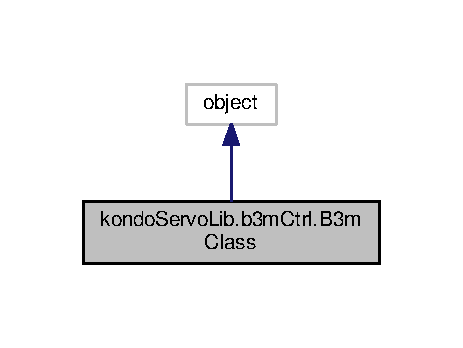
\includegraphics[width=222pt]{classkondoServoLib_1_1b3mCtrl_1_1B3mClass__inherit__graph}
\end{center}
\end{figure}


Collaboration diagram for kondo\+Servo\+Lib.\+b3m\+Ctrl.\+B3m\+Class\+:\nopagebreak
\begin{figure}[H]
\begin{center}
\leavevmode
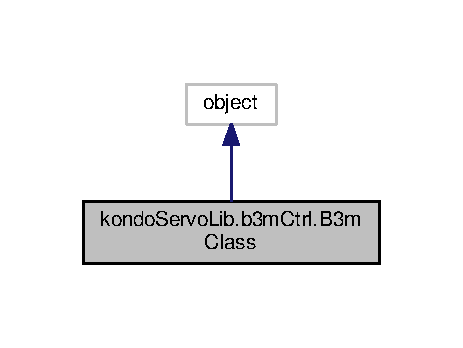
\includegraphics[width=222pt]{classkondoServoLib_1_1b3mCtrl_1_1B3mClass__coll__graph}
\end{center}
\end{figure}
\subsection*{Public Member Functions}
\begin{DoxyCompactItemize}
\item 
def {\bfseries \+\_\+\+\_\+init\+\_\+\+\_\+} (self, \+\_\+port=None, \+\_\+baudrate=1500000, \+\_\+timeout=0.\+005)\hypertarget{classkondoServoLib_1_1b3mCtrl_1_1B3mClass_ab28360948b42d79f03158051877ca954}{}\label{classkondoServoLib_1_1b3mCtrl_1_1B3mClass_ab28360948b42d79f03158051877ca954}

\item 
def {\bfseries \+\_\+\+\_\+del\+\_\+\+\_\+} (self)\hypertarget{classkondoServoLib_1_1b3mCtrl_1_1B3mClass_aba9380d00c91d145ef00f13b9d7d76a7}{}\label{classkondoServoLib_1_1b3mCtrl_1_1B3mClass_aba9380d00c91d145ef00f13b9d7d76a7}

\item 
def \hyperlink{classkondoServoLib_1_1b3mCtrl_1_1B3mClass_a0011e73a24e0f0ece31b4297ac0b1312}{begin} (self, \+\_\+port=None, \+\_\+baudrate=None, \+\_\+timeout=None)
\begin{DoxyCompactList}\small\item\em 通信開始設定 \end{DoxyCompactList}\item 
def \hyperlink{classkondoServoLib_1_1b3mCtrl_1_1B3mClass_a8a8d8a892485a9aa537851e08311b9b7}{load\+Cmd} (self, id, option=\char`\"{}E\+R\+R\+OR\char`\"{})
\begin{DoxyCompactList}\small\item\em R\+O\+Mを\+R\+A\+Mに書き込み(シングル/マルチ) \end{DoxyCompactList}\item 
def \hyperlink{classkondoServoLib_1_1b3mCtrl_1_1B3mClass_a4455a0ce6b75651328ddfe49360891dc}{save\+Cmd} (self, id, option=\char`\"{}E\+R\+R\+OR\char`\"{})
\begin{DoxyCompactList}\small\item\em R\+A\+Mを\+R\+O\+Mに書き込み(シングル/マルチ) \end{DoxyCompactList}\item 
def \hyperlink{classkondoServoLib_1_1b3mCtrl_1_1B3mClass_abf799c4dd10d66f48801326c7cf44372}{read\+Cmd} (self, id, address, length, option=\char`\"{}E\+R\+R\+OR\char`\"{})
\begin{DoxyCompactList}\small\item\em R\+A\+Mの読み出し(シングル) \end{DoxyCompactList}\item 
def \hyperlink{classkondoServoLib_1_1b3mCtrl_1_1B3mClass_ab5e0a4218a091ba3a499da7dcd14b31a}{write\+Cmd} (self, id, address, data, option=\char`\"{}E\+R\+R\+OR\char`\"{})
\begin{DoxyCompactList}\small\item\em R\+A\+Mへの書き込み(シングル/マルチ) \end{DoxyCompactList}\item 
def \hyperlink{classkondoServoLib_1_1b3mCtrl_1_1B3mClass_aa8a3a74d41ac831954b8a01d6f487c8a}{reset\+Cmd} (self, id, time=0, option=\char`\"{}E\+R\+R\+OR\char`\"{})
\begin{DoxyCompactList}\small\item\em 再起動要求(シングル/マルチ) \end{DoxyCompactList}\item 
def \hyperlink{classkondoServoLib_1_1b3mCtrl_1_1B3mClass_ad4eb38a1437ddae5888aeb2c34b6a813}{position\+Cmd} (self, id, pos, time=0, option=\char`\"{}E\+R\+R\+OR\char`\"{})
\begin{DoxyCompactList}\small\item\em 位置設定(シングル/マルチ) \end{DoxyCompactList}\item 
def {\bfseries set\+Mode} (self, id, mode, option=\char`\"{}E\+R\+R\+OR\char`\"{})\hypertarget{classkondoServoLib_1_1b3mCtrl_1_1B3mClass_adf996502303aa487f4053f116a53432a}{}\label{classkondoServoLib_1_1b3mCtrl_1_1B3mClass_adf996502303aa487f4053f116a53432a}

\item 
def {\bfseries set\+Trajectory\+Type} (self, id, \+\_\+type, option=\char`\"{}E\+R\+R\+OR\char`\"{})\hypertarget{classkondoServoLib_1_1b3mCtrl_1_1B3mClass_a80d952179d4a163bf940327838295dd1}{}\label{classkondoServoLib_1_1b3mCtrl_1_1B3mClass_a80d952179d4a163bf940327838295dd1}

\item 
def {\bfseries set\+Ram} (self, id, data, property, option=\char`\"{}E\+R\+R\+OR\char`\"{})\hypertarget{classkondoServoLib_1_1b3mCtrl_1_1B3mClass_a3df6bc15e8c68b876ab9af208ee6ffb0}{}\label{classkondoServoLib_1_1b3mCtrl_1_1B3mClass_a3df6bc15e8c68b876ab9af208ee6ffb0}

\item 
def {\bfseries get\+Ram} (self, id, property, option=\char`\"{}E\+R\+R\+OR\char`\"{})\hypertarget{classkondoServoLib_1_1b3mCtrl_1_1B3mClass_a556267ec8a99ea44fce091c61d3c53b6}{}\label{classkondoServoLib_1_1b3mCtrl_1_1B3mClass_a556267ec8a99ea44fce091c61d3c53b6}

\item 
def {\bfseries set\+New\+Id} (self, current\+Id, new\+Id)\hypertarget{classkondoServoLib_1_1b3mCtrl_1_1B3mClass_ab8e85e88765bc5476e34bf2e9fa07527}{}\label{classkondoServoLib_1_1b3mCtrl_1_1B3mClass_ab8e85e88765bc5476e34bf2e9fa07527}

\end{DoxyCompactItemize}
\subsection*{Static Public Member Functions}
\begin{DoxyCompactItemize}
\item 
def {\bfseries deg\+To\+Pos} (deg)\hypertarget{classkondoServoLib_1_1b3mCtrl_1_1B3mClass_ab1c79f3b27609003cf8896b58b2aba5a}{}\label{classkondoServoLib_1_1b3mCtrl_1_1B3mClass_ab1c79f3b27609003cf8896b58b2aba5a}

\item 
def {\bfseries pos\+To\+Deg} (pos)\hypertarget{classkondoServoLib_1_1b3mCtrl_1_1B3mClass_ad0b48cf19eb33b2e9008c16ae8d49002}{}\label{classkondoServoLib_1_1b3mCtrl_1_1B3mClass_ad0b48cf19eb33b2e9008c16ae8d49002}

\item 
def {\bfseries rad\+To\+Pos} (rad)\hypertarget{classkondoServoLib_1_1b3mCtrl_1_1B3mClass_aacc7f359bec5b5117c187fb22e2417b6}{}\label{classkondoServoLib_1_1b3mCtrl_1_1B3mClass_aacc7f359bec5b5117c187fb22e2417b6}

\item 
def {\bfseries pos\+To\+Rad} (pos)\hypertarget{classkondoServoLib_1_1b3mCtrl_1_1B3mClass_a96ed8d1b0059d8523c0096e75aa3a352}{}\label{classkondoServoLib_1_1b3mCtrl_1_1B3mClass_a96ed8d1b0059d8523c0096e75aa3a352}

\end{DoxyCompactItemize}
\subsection*{Public Attributes}
\begin{DoxyCompactItemize}
\item 
{\bfseries port}\hypertarget{classkondoServoLib_1_1b3mCtrl_1_1B3mClass_afce4612ca370673aae07649868e57386}{}\label{classkondoServoLib_1_1b3mCtrl_1_1B3mClass_afce4612ca370673aae07649868e57386}

\item 
{\bfseries baudrate}\hypertarget{classkondoServoLib_1_1b3mCtrl_1_1B3mClass_a2e589066c3f3f08af5f1ef1779b0b192}{}\label{classkondoServoLib_1_1b3mCtrl_1_1B3mClass_a2e589066c3f3f08af5f1ef1779b0b192}

\item 
{\bfseries timeout}\hypertarget{classkondoServoLib_1_1b3mCtrl_1_1B3mClass_a4ced53ee2019d71f41caf7540915cc7e}{}\label{classkondoServoLib_1_1b3mCtrl_1_1B3mClass_a4ced53ee2019d71f41caf7540915cc7e}

\item 
{\bfseries last\+Snyc\+End\+Time}\hypertarget{classkondoServoLib_1_1b3mCtrl_1_1B3mClass_ac0edaa150cbd1a0d6a3d5582568449bf}{}\label{classkondoServoLib_1_1b3mCtrl_1_1B3mClass_ac0edaa150cbd1a0d6a3d5582568449bf}

\item 
{\bfseries receive\+Len\+Plan}\hypertarget{classkondoServoLib_1_1b3mCtrl_1_1B3mClass_ac83d747fb138aded4ad4c35cf1206ebf}{}\label{classkondoServoLib_1_1b3mCtrl_1_1B3mClass_ac83d747fb138aded4ad4c35cf1206ebf}

\item 
{\bfseries gard\+Time}\hypertarget{classkondoServoLib_1_1b3mCtrl_1_1B3mClass_a2eecf362e6824da5dbef84eba18101ce}{}\label{classkondoServoLib_1_1b3mCtrl_1_1B3mClass_a2eecf362e6824da5dbef84eba18101ce}

\item 
{\bfseries b3m\+Serial}\hypertarget{classkondoServoLib_1_1b3mCtrl_1_1B3mClass_aefd7aa4627d0b41d80ec44e6602ba853}{}\label{classkondoServoLib_1_1b3mCtrl_1_1B3mClass_aefd7aa4627d0b41d80ec44e6602ba853}

\end{DoxyCompactItemize}
\subsection*{Static Public Attributes}
\begin{DoxyCompactItemize}
\item 
int {\bfseries M\+A\+X\+\_\+\+ID} = 255\hypertarget{classkondoServoLib_1_1b3mCtrl_1_1B3mClass_a92c5da3a7168857ea770078574132290}{}\label{classkondoServoLib_1_1b3mCtrl_1_1B3mClass_a92c5da3a7168857ea770078574132290}

\item 
int {\bfseries M\+I\+N\+\_\+\+ID} = 0\hypertarget{classkondoServoLib_1_1b3mCtrl_1_1B3mClass_a3503c1076faba33710746d3618c57e0d}{}\label{classkondoServoLib_1_1b3mCtrl_1_1B3mClass_a3503c1076faba33710746d3618c57e0d}

\item 
int {\bfseries M\+A\+X\+\_\+\+P\+OS} = 32000\hypertarget{classkondoServoLib_1_1b3mCtrl_1_1B3mClass_a70d773fe1e2ccfb6a955110140cf0a59}{}\label{classkondoServoLib_1_1b3mCtrl_1_1B3mClass_a70d773fe1e2ccfb6a955110140cf0a59}

\item 
int {\bfseries M\+I\+N\+\_\+\+P\+OS} = -\/32000\hypertarget{classkondoServoLib_1_1b3mCtrl_1_1B3mClass_a29f228cf17efb8c5f48180dc485c5cae}{}\label{classkondoServoLib_1_1b3mCtrl_1_1B3mClass_a29f228cf17efb8c5f48180dc485c5cae}

\item 
dictionary {\bfseries M\+E\+M\+O\+R\+Y\+\_\+\+M\+AP}\hypertarget{classkondoServoLib_1_1b3mCtrl_1_1B3mClass_a71883622fe29913c6f899129c39681b4}{}\label{classkondoServoLib_1_1b3mCtrl_1_1B3mClass_a71883622fe29913c6f899129c39681b4}

\end{DoxyCompactItemize}


\subsection{Member Function Documentation}
\index{kondo\+Servo\+Lib\+::b3m\+Ctrl\+::\+B3m\+Class@{kondo\+Servo\+Lib\+::b3m\+Ctrl\+::\+B3m\+Class}!begin@{begin}}
\index{begin@{begin}!kondo\+Servo\+Lib\+::b3m\+Ctrl\+::\+B3m\+Class@{kondo\+Servo\+Lib\+::b3m\+Ctrl\+::\+B3m\+Class}}
\subsubsection[{\texorpdfstring{begin(self, \+\_\+port=\+None, \+\_\+baudrate=\+None, \+\_\+timeout=\+None)}{begin(self, _port=None, _baudrate=None, _timeout=None)}}]{\setlength{\rightskip}{0pt plus 5cm}def kondo\+Servo\+Lib.\+b3m\+Ctrl.\+B3m\+Class.\+begin (
\begin{DoxyParamCaption}
\item[{}]{self, }
\item[{}]{\+\_\+port = {\ttfamily None}, }
\item[{}]{\+\_\+baudrate = {\ttfamily None}, }
\item[{}]{\+\_\+timeout = {\ttfamily None}}
\end{DoxyParamCaption}
)}\hypertarget{classkondoServoLib_1_1b3mCtrl_1_1B3mClass_a0011e73a24e0f0ece31b4297ac0b1312}{}\label{classkondoServoLib_1_1b3mCtrl_1_1B3mClass_a0011e73a24e0f0ece31b4297ac0b1312}


通信開始設定 


\begin{DoxyParams}{Parameters}
{\em \+\_\+port(str)} & = デバイス名 \\
\hline
{\em \+\_\+baudrate(int)} & = 通信速度 \\
\hline
{\em \+\_\+timeout(float)} & = 受信待ちタイムアウト時間 \\
\hline
\end{DoxyParams}
\index{kondo\+Servo\+Lib\+::b3m\+Ctrl\+::\+B3m\+Class@{kondo\+Servo\+Lib\+::b3m\+Ctrl\+::\+B3m\+Class}!load\+Cmd@{load\+Cmd}}
\index{load\+Cmd@{load\+Cmd}!kondo\+Servo\+Lib\+::b3m\+Ctrl\+::\+B3m\+Class@{kondo\+Servo\+Lib\+::b3m\+Ctrl\+::\+B3m\+Class}}
\subsubsection[{\texorpdfstring{load\+Cmd(self, id, option=""E\+R\+R\+OR"")}{loadCmd(self, id, option="ERROR")}}]{\setlength{\rightskip}{0pt plus 5cm}def kondo\+Servo\+Lib.\+b3m\+Ctrl.\+B3m\+Class.\+load\+Cmd (
\begin{DoxyParamCaption}
\item[{}]{self, }
\item[{}]{id, }
\item[{}]{option = {\ttfamily \char`\"{}ERROR\char`\"{}}}
\end{DoxyParamCaption}
)}\hypertarget{classkondoServoLib_1_1b3mCtrl_1_1B3mClass_a8a8d8a892485a9aa537851e08311b9b7}{}\label{classkondoServoLib_1_1b3mCtrl_1_1B3mClass_a8a8d8a892485a9aa537851e08311b9b7}


R\+O\+Mを\+R\+A\+Mに書き込み(シングル/マルチ) 


\begin{DoxyParams}{Parameters}
{\em id(int)} & = サーボ\+ID(シングル) \\
\hline
{\em id(list)} & = サーボ\+ID(マルチ) \\
\hline
{\em option(str)} & = 返値オプション \\
\hline
\end{DoxyParams}
\begin{DoxyReturn}{Returns}
成功(tuple) = (True, ステータス) 

失敗(tuple) = (False, False) 
\end{DoxyReturn}
\index{kondo\+Servo\+Lib\+::b3m\+Ctrl\+::\+B3m\+Class@{kondo\+Servo\+Lib\+::b3m\+Ctrl\+::\+B3m\+Class}!position\+Cmd@{position\+Cmd}}
\index{position\+Cmd@{position\+Cmd}!kondo\+Servo\+Lib\+::b3m\+Ctrl\+::\+B3m\+Class@{kondo\+Servo\+Lib\+::b3m\+Ctrl\+::\+B3m\+Class}}
\subsubsection[{\texorpdfstring{position\+Cmd(self, id, pos, time=0, option=""E\+R\+R\+OR"")}{positionCmd(self, id, pos, time=0, option="ERROR")}}]{\setlength{\rightskip}{0pt plus 5cm}def kondo\+Servo\+Lib.\+b3m\+Ctrl.\+B3m\+Class.\+position\+Cmd (
\begin{DoxyParamCaption}
\item[{}]{self, }
\item[{}]{id, }
\item[{}]{pos, }
\item[{}]{time = {\ttfamily 0}, }
\item[{}]{option = {\ttfamily \char`\"{}ERROR\char`\"{}}}
\end{DoxyParamCaption}
)}\hypertarget{classkondoServoLib_1_1b3mCtrl_1_1B3mClass_ad4eb38a1437ddae5888aeb2c34b6a813}{}\label{classkondoServoLib_1_1b3mCtrl_1_1B3mClass_ad4eb38a1437ddae5888aeb2c34b6a813}


位置設定(シングル/マルチ) 


\begin{DoxyParams}{Parameters}
{\em id(int)} & = サーボ\+ID(シングル) \\
\hline
{\em id(list)} & = サーボ\+ID(マルチ) \\
\hline
{\em pos(float)} & = 目標位置\mbox{[}rad\mbox{]} \\
\hline
{\em pos(list)} & = 目標位置\mbox{[}rad\mbox{]} \\
\hline
{\em time(float)} & = 移動完了目標時間\mbox{[}sec\mbox{]} \\
\hline
{\em option(str)} & = 返値オプション \\
\hline
\end{DoxyParams}
\begin{DoxyReturn}{Returns}
成否(bool) 
\end{DoxyReturn}
\index{kondo\+Servo\+Lib\+::b3m\+Ctrl\+::\+B3m\+Class@{kondo\+Servo\+Lib\+::b3m\+Ctrl\+::\+B3m\+Class}!read\+Cmd@{read\+Cmd}}
\index{read\+Cmd@{read\+Cmd}!kondo\+Servo\+Lib\+::b3m\+Ctrl\+::\+B3m\+Class@{kondo\+Servo\+Lib\+::b3m\+Ctrl\+::\+B3m\+Class}}
\subsubsection[{\texorpdfstring{read\+Cmd(self, id, address, length, option=""E\+R\+R\+OR"")}{readCmd(self, id, address, length, option="ERROR")}}]{\setlength{\rightskip}{0pt plus 5cm}def kondo\+Servo\+Lib.\+b3m\+Ctrl.\+B3m\+Class.\+read\+Cmd (
\begin{DoxyParamCaption}
\item[{}]{self, }
\item[{}]{id, }
\item[{}]{address, }
\item[{}]{length, }
\item[{}]{option = {\ttfamily \char`\"{}ERROR\char`\"{}}}
\end{DoxyParamCaption}
)}\hypertarget{classkondoServoLib_1_1b3mCtrl_1_1B3mClass_abf799c4dd10d66f48801326c7cf44372}{}\label{classkondoServoLib_1_1b3mCtrl_1_1B3mClass_abf799c4dd10d66f48801326c7cf44372}


R\+A\+Mの読み出し(シングル) 


\begin{DoxyParams}{Parameters}
{\em id(int)} & = サーボ\+ID \\
\hline
{\em address(int)} & = 読み込みアドレス \\
\hline
{\em length(int)} & = 読み込みデータ長さ \\
\hline
{\em option(str)} & = 返値オプション \\
\hline
\end{DoxyParams}
\begin{DoxyReturn}{Returns}
成功(tuple) = (R\+A\+Mデータ, ステータス) 

失敗(tuple) = (False, False) 
\end{DoxyReturn}
\index{kondo\+Servo\+Lib\+::b3m\+Ctrl\+::\+B3m\+Class@{kondo\+Servo\+Lib\+::b3m\+Ctrl\+::\+B3m\+Class}!reset\+Cmd@{reset\+Cmd}}
\index{reset\+Cmd@{reset\+Cmd}!kondo\+Servo\+Lib\+::b3m\+Ctrl\+::\+B3m\+Class@{kondo\+Servo\+Lib\+::b3m\+Ctrl\+::\+B3m\+Class}}
\subsubsection[{\texorpdfstring{reset\+Cmd(self, id, time=0, option=""E\+R\+R\+OR"")}{resetCmd(self, id, time=0, option="ERROR")}}]{\setlength{\rightskip}{0pt plus 5cm}def kondo\+Servo\+Lib.\+b3m\+Ctrl.\+B3m\+Class.\+reset\+Cmd (
\begin{DoxyParamCaption}
\item[{}]{self, }
\item[{}]{id, }
\item[{}]{time = {\ttfamily 0}, }
\item[{}]{option = {\ttfamily \char`\"{}ERROR\char`\"{}}}
\end{DoxyParamCaption}
)}\hypertarget{classkondoServoLib_1_1b3mCtrl_1_1B3mClass_aa8a3a74d41ac831954b8a01d6f487c8a}{}\label{classkondoServoLib_1_1b3mCtrl_1_1B3mClass_aa8a3a74d41ac831954b8a01d6f487c8a}


再起動要求(シングル/マルチ) 


\begin{DoxyParams}{Parameters}
{\em id(int)} & = サーボ\+ID(シングル) \\
\hline
{\em id(list)} & = サーボ\+ID(マルチ) \\
\hline
{\em time(float)} & = 再起動遅延時間(sec) \\
\hline
{\em option(str)} & = 返値オプション \\
\hline
\end{DoxyParams}
\begin{DoxyReturn}{Returns}
成否(bool) 
\end{DoxyReturn}
\index{kondo\+Servo\+Lib\+::b3m\+Ctrl\+::\+B3m\+Class@{kondo\+Servo\+Lib\+::b3m\+Ctrl\+::\+B3m\+Class}!save\+Cmd@{save\+Cmd}}
\index{save\+Cmd@{save\+Cmd}!kondo\+Servo\+Lib\+::b3m\+Ctrl\+::\+B3m\+Class@{kondo\+Servo\+Lib\+::b3m\+Ctrl\+::\+B3m\+Class}}
\subsubsection[{\texorpdfstring{save\+Cmd(self, id, option=""E\+R\+R\+OR"")}{saveCmd(self, id, option="ERROR")}}]{\setlength{\rightskip}{0pt plus 5cm}def kondo\+Servo\+Lib.\+b3m\+Ctrl.\+B3m\+Class.\+save\+Cmd (
\begin{DoxyParamCaption}
\item[{}]{self, }
\item[{}]{id, }
\item[{}]{option = {\ttfamily \char`\"{}ERROR\char`\"{}}}
\end{DoxyParamCaption}
)}\hypertarget{classkondoServoLib_1_1b3mCtrl_1_1B3mClass_a4455a0ce6b75651328ddfe49360891dc}{}\label{classkondoServoLib_1_1b3mCtrl_1_1B3mClass_a4455a0ce6b75651328ddfe49360891dc}


R\+A\+Mを\+R\+O\+Mに書き込み(シングル/マルチ) 


\begin{DoxyParams}{Parameters}
{\em id(int)} & = サーボ\+ID(シングル) \\
\hline
{\em id(list)} & = サーボ\+ID(マルチ) \\
\hline
{\em option(str)} & = 返値オプション \\
\hline
\end{DoxyParams}
\begin{DoxyReturn}{Returns}
成功(tuple) = (True, True) 

失敗(tuple) = (False, False) 
\end{DoxyReturn}
\index{kondo\+Servo\+Lib\+::b3m\+Ctrl\+::\+B3m\+Class@{kondo\+Servo\+Lib\+::b3m\+Ctrl\+::\+B3m\+Class}!write\+Cmd@{write\+Cmd}}
\index{write\+Cmd@{write\+Cmd}!kondo\+Servo\+Lib\+::b3m\+Ctrl\+::\+B3m\+Class@{kondo\+Servo\+Lib\+::b3m\+Ctrl\+::\+B3m\+Class}}
\subsubsection[{\texorpdfstring{write\+Cmd(self, id, address, data, option=""E\+R\+R\+OR"")}{writeCmd(self, id, address, data, option="ERROR")}}]{\setlength{\rightskip}{0pt plus 5cm}def kondo\+Servo\+Lib.\+b3m\+Ctrl.\+B3m\+Class.\+write\+Cmd (
\begin{DoxyParamCaption}
\item[{}]{self, }
\item[{}]{id, }
\item[{}]{address, }
\item[{}]{data, }
\item[{}]{option = {\ttfamily \char`\"{}ERROR\char`\"{}}}
\end{DoxyParamCaption}
)}\hypertarget{classkondoServoLib_1_1b3mCtrl_1_1B3mClass_ab5e0a4218a091ba3a499da7dcd14b31a}{}\label{classkondoServoLib_1_1b3mCtrl_1_1B3mClass_ab5e0a4218a091ba3a499da7dcd14b31a}


R\+A\+Mへの書き込み(シングル/マルチ) 


\begin{DoxyParams}{Parameters}
{\em id(int)} & = サーボ\+ID(シングル) \\
\hline
{\em id(list)} & = サーボ\+ID(マルチ) \\
\hline
{\em address(int)} & = 書き込みアドレス \\
\hline
{\em data(list)} & = 書き込みデータ(シングル) \\
\hline
{\em data(list\+\_\+of\+\_\+list)} & = 書き込みデータ(マルチ) ~\newline
 例)data次元数 = idの次元数+1 id=\mbox{[}1,2,3\mbox{]} data=\mbox{[}\mbox{[}10,20\mbox{]}, \mbox{[}100,200\mbox{]}, \mbox{[}1000,2000\mbox{]}\mbox{]} \\
\hline
{\em option(str)} & = 返値オプション \\
\hline
\end{DoxyParams}
\begin{DoxyReturn}{Returns}
シングル成功(tuple) = (R\+A\+Mデータ, ステータス) 

マルチ成功(tuple) = (True, True) 

失敗(tuple) = (False, False) 
\end{DoxyReturn}


The documentation for this class was generated from the following file\+:\begin{DoxyCompactItemize}
\item 
b3m\+Ctrl.\+py\end{DoxyCompactItemize}

\hypertarget{classkondoServoLib_1_1ctrlKondoServo_1_1ctrlKondoServoClass}{}\section{kondo\+Servo\+Lib.\+ctrl\+Kondo\+Servo.\+ctrl\+Kondo\+Servo\+Class Class Reference}
\label{classkondoServoLib_1_1ctrlKondoServo_1_1ctrlKondoServoClass}\index{kondo\+Servo\+Lib.\+ctrl\+Kondo\+Servo.\+ctrl\+Kondo\+Servo\+Class@{kondo\+Servo\+Lib.\+ctrl\+Kondo\+Servo.\+ctrl\+Kondo\+Servo\+Class}}
\subsection*{Public Member Functions}
\begin{DoxyCompactItemize}
\item 
def {\bfseries \+\_\+\+\_\+init\+\_\+\+\_\+} (self, \+\_\+ics\+Port, \+\_\+b3m\+Port)\hypertarget{classkondoServoLib_1_1ctrlKondoServo_1_1ctrlKondoServoClass_a7a6811cf4a66dd452a36dab58726bb86}{}\label{classkondoServoLib_1_1ctrlKondoServo_1_1ctrlKondoServoClass_a7a6811cf4a66dd452a36dab58726bb86}

\item 
def {\bfseries begin\+B3m} (self, id\+List, speed=1500000)\hypertarget{classkondoServoLib_1_1ctrlKondoServo_1_1ctrlKondoServoClass_a6f6de909a0ece5d8b079af5ddc6403ad}{}\label{classkondoServoLib_1_1ctrlKondoServo_1_1ctrlKondoServoClass_a6f6de909a0ece5d8b079af5ddc6403ad}

\item 
def {\bfseries begin\+Ics} (self, id\+List, speed=115200)\hypertarget{classkondoServoLib_1_1ctrlKondoServo_1_1ctrlKondoServoClass_acc8581a2fb8a1f571cc54b01b01f9fda}{}\label{classkondoServoLib_1_1ctrlKondoServo_1_1ctrlKondoServoClass_acc8581a2fb8a1f571cc54b01b01f9fda}

\item 
def {\bfseries learn\+Joint\+Name} (self, joint\+Name, id, B3\+Mor\+I\+CS)\hypertarget{classkondoServoLib_1_1ctrlKondoServo_1_1ctrlKondoServoClass_a816e29c997c82145b828e91b0a3a4a5e}{}\label{classkondoServoLib_1_1ctrlKondoServo_1_1ctrlKondoServoClass_a816e29c997c82145b828e91b0a3a4a5e}

\item 
def {\bfseries drive\+Joint} (self, servo, angle, time=0)\hypertarget{classkondoServoLib_1_1ctrlKondoServo_1_1ctrlKondoServoClass_a624954b797bfbc0029f5f842ebeea54d}{}\label{classkondoServoLib_1_1ctrlKondoServo_1_1ctrlKondoServoClass_a624954b797bfbc0029f5f842ebeea54d}

\item 
def {\bfseries drive\+Joint\+State} (self, joint\+State, sec=0)\hypertarget{classkondoServoLib_1_1ctrlKondoServo_1_1ctrlKondoServoClass_afb7c033773f11e85b09bf5ed8c025cc4}{}\label{classkondoServoLib_1_1ctrlKondoServo_1_1ctrlKondoServoClass_afb7c033773f11e85b09bf5ed8c025cc4}

\item 
def {\bfseries drive\+Plan} (self, robot\+Trajectory)\hypertarget{classkondoServoLib_1_1ctrlKondoServo_1_1ctrlKondoServoClass_ae336530b8f316c9726dd80ffc266f80c}{}\label{classkondoServoLib_1_1ctrlKondoServo_1_1ctrlKondoServoClass_ae336530b8f316c9726dd80ffc266f80c}

\item 
def {\bfseries free\+Joint} (self, servo)\hypertarget{classkondoServoLib_1_1ctrlKondoServo_1_1ctrlKondoServoClass_a25671a317480446ac56af76f7bf2a7da}{}\label{classkondoServoLib_1_1ctrlKondoServo_1_1ctrlKondoServoClass_a25671a317480446ac56af76f7bf2a7da}

\item 
def {\bfseries get\+Pos\+Joint} (self, servo)\hypertarget{classkondoServoLib_1_1ctrlKondoServo_1_1ctrlKondoServoClass_ae3d7ca6568f4d54fe47461bdf683a7ce}{}\label{classkondoServoLib_1_1ctrlKondoServo_1_1ctrlKondoServoClass_ae3d7ca6568f4d54fe47461bdf683a7ce}

\end{DoxyCompactItemize}
\subsection*{Public Attributes}
\begin{DoxyCompactItemize}
\item 
{\bfseries ics\+Port}\hypertarget{classkondoServoLib_1_1ctrlKondoServo_1_1ctrlKondoServoClass_a23932f86ffca0a44ffb4f4d1eb76fe7d}{}\label{classkondoServoLib_1_1ctrlKondoServo_1_1ctrlKondoServoClass_a23932f86ffca0a44ffb4f4d1eb76fe7d}

\item 
{\bfseries b3m\+Port}\hypertarget{classkondoServoLib_1_1ctrlKondoServo_1_1ctrlKondoServoClass_a7bf60306d45b4fc8e545bf890db01f1c}{}\label{classkondoServoLib_1_1ctrlKondoServo_1_1ctrlKondoServoClass_a7bf60306d45b4fc8e545bf890db01f1c}

\item 
{\bfseries joint\+Name\+To\+Id\+Dict}\hypertarget{classkondoServoLib_1_1ctrlKondoServo_1_1ctrlKondoServoClass_a10192ad62812e223dc06f78f332c8557}{}\label{classkondoServoLib_1_1ctrlKondoServo_1_1ctrlKondoServoClass_a10192ad62812e223dc06f78f332c8557}

\item 
{\bfseries id\+To\+Servo\+Type\+Dict}\hypertarget{classkondoServoLib_1_1ctrlKondoServo_1_1ctrlKondoServoClass_abab034fba95ef3a6c074af8799ddd3a2}{}\label{classkondoServoLib_1_1ctrlKondoServo_1_1ctrlKondoServoClass_abab034fba95ef3a6c074af8799ddd3a2}

\item 
{\bfseries id\+To\+B3m\+Mode\+Dict}\hypertarget{classkondoServoLib_1_1ctrlKondoServo_1_1ctrlKondoServoClass_a7b265836bb5f9b888ed6745eff1f9f09}{}\label{classkondoServoLib_1_1ctrlKondoServo_1_1ctrlKondoServoClass_a7b265836bb5f9b888ed6745eff1f9f09}

\item 
{\bfseries id\+To\+Ics\+Last\+Send\+Pos}\hypertarget{classkondoServoLib_1_1ctrlKondoServo_1_1ctrlKondoServoClass_a78cf91e3cd0c329c98590322f1fc6f0e}{}\label{classkondoServoLib_1_1ctrlKondoServo_1_1ctrlKondoServoClass_a78cf91e3cd0c329c98590322f1fc6f0e}

\item 
{\bfseries B3m}\hypertarget{classkondoServoLib_1_1ctrlKondoServo_1_1ctrlKondoServoClass_afde3561fccfb416aac22502c54b67397}{}\label{classkondoServoLib_1_1ctrlKondoServo_1_1ctrlKondoServoClass_afde3561fccfb416aac22502c54b67397}

\item 
{\bfseries Ics}\hypertarget{classkondoServoLib_1_1ctrlKondoServo_1_1ctrlKondoServoClass_a9bd75eb55622512c776b500ede5e96be}{}\label{classkondoServoLib_1_1ctrlKondoServo_1_1ctrlKondoServoClass_a9bd75eb55622512c776b500ede5e96be}

\end{DoxyCompactItemize}


The documentation for this class was generated from the following file\+:\begin{DoxyCompactItemize}
\item 
ctrl\+Kondo\+Servo.\+py\end{DoxyCompactItemize}

\hypertarget{classkondoServoLib_1_1icsCtrl_1_1IcsClass}{}\section{kondo\+Servo\+Lib.\+ics\+Ctrl.\+Ics\+Class Class Reference}
\label{classkondoServoLib_1_1icsCtrl_1_1IcsClass}\index{kondo\+Servo\+Lib.\+ics\+Ctrl.\+Ics\+Class@{kondo\+Servo\+Lib.\+ics\+Ctrl.\+Ics\+Class}}


Inheritance diagram for kondo\+Servo\+Lib.\+ics\+Ctrl.\+Ics\+Class\+:\nopagebreak
\begin{figure}[H]
\begin{center}
\leavevmode
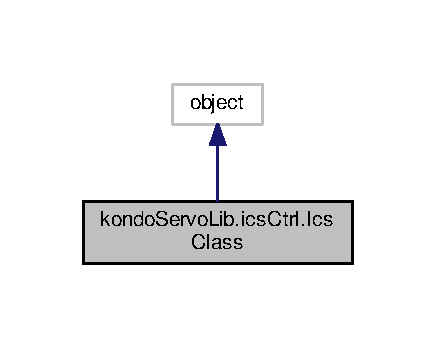
\includegraphics[width=209pt]{classkondoServoLib_1_1icsCtrl_1_1IcsClass__inherit__graph}
\end{center}
\end{figure}


Collaboration diagram for kondo\+Servo\+Lib.\+ics\+Ctrl.\+Ics\+Class\+:\nopagebreak
\begin{figure}[H]
\begin{center}
\leavevmode
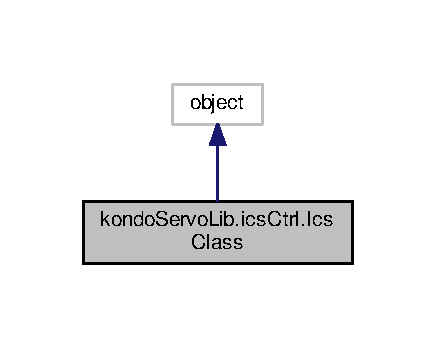
\includegraphics[width=209pt]{classkondoServoLib_1_1icsCtrl_1_1IcsClass__coll__graph}
\end{center}
\end{figure}
\subsection*{Public Member Functions}
\begin{DoxyCompactItemize}
\item 
def {\bfseries \+\_\+\+\_\+init\+\_\+\+\_\+} (self, \+\_\+port=None, \+\_\+baudrate=115200, \+\_\+timeout=0.\+02)\hypertarget{classkondoServoLib_1_1icsCtrl_1_1IcsClass_a406e99d98fe5ce6181fc3ae3bf4a530a}{}\label{classkondoServoLib_1_1icsCtrl_1_1IcsClass_a406e99d98fe5ce6181fc3ae3bf4a530a}

\item 
def {\bfseries \+\_\+\+\_\+del\+\_\+\+\_\+} (self)\hypertarget{classkondoServoLib_1_1icsCtrl_1_1IcsClass_a3e9191c28f5cccec5c5bcd999193038b}{}\label{classkondoServoLib_1_1icsCtrl_1_1IcsClass_a3e9191c28f5cccec5c5bcd999193038b}

\item 
def {\bfseries begin} (self, \+\_\+port=None, \+\_\+baudrate=None, \+\_\+timeout=None)\hypertarget{classkondoServoLib_1_1icsCtrl_1_1IcsClass_a9fbca8361c052597d207a95397f4ca38}{}\label{classkondoServoLib_1_1icsCtrl_1_1IcsClass_a9fbca8361c052597d207a95397f4ca38}

\item 
def {\bfseries read\+Cmd} (self, id, sub\+Cmd)\hypertarget{classkondoServoLib_1_1icsCtrl_1_1IcsClass_a0d65ad4731c502b5e2297ac278ef6570}{}\label{classkondoServoLib_1_1icsCtrl_1_1IcsClass_a0d65ad4731c502b5e2297ac278ef6570}

\item 
def {\bfseries write\+Cmd} (self, id, sub\+Cmd, data)\hypertarget{classkondoServoLib_1_1icsCtrl_1_1IcsClass_a4800d3a988f701ea747a621687364421}{}\label{classkondoServoLib_1_1icsCtrl_1_1IcsClass_a4800d3a988f701ea747a621687364421}

\item 
def {\bfseries id\+Cmd} (self, id, RorW)\hypertarget{classkondoServoLib_1_1icsCtrl_1_1IcsClass_a0d6981c5d3ef401dd3b9951e841103ad}{}\label{classkondoServoLib_1_1icsCtrl_1_1IcsClass_a0d6981c5d3ef401dd3b9951e841103ad}

\item 
def {\bfseries set\+Pos} (self, id, pos)\hypertarget{classkondoServoLib_1_1icsCtrl_1_1IcsClass_a94a5f6a77f91b645667956919bfcf345}{}\label{classkondoServoLib_1_1icsCtrl_1_1IcsClass_a94a5f6a77f91b645667956919bfcf345}

\item 
def {\bfseries set\+Free} (self, id)\hypertarget{classkondoServoLib_1_1icsCtrl_1_1IcsClass_a406e9746deb4acb4bbafddc7a1f93f6e}{}\label{classkondoServoLib_1_1icsCtrl_1_1IcsClass_a406e9746deb4acb4bbafddc7a1f93f6e}

\item 
def {\bfseries set\+Strc} (self, id, strc)\hypertarget{classkondoServoLib_1_1icsCtrl_1_1IcsClass_a70a3eb9d22403d60855be0606f5e5574}{}\label{classkondoServoLib_1_1icsCtrl_1_1IcsClass_a70a3eb9d22403d60855be0606f5e5574}

\item 
def {\bfseries set\+Spd} (self, id, spd)\hypertarget{classkondoServoLib_1_1icsCtrl_1_1IcsClass_a2507a327f61fd2ebe071c1986d60d827}{}\label{classkondoServoLib_1_1icsCtrl_1_1IcsClass_a2507a327f61fd2ebe071c1986d60d827}

\item 
def {\bfseries set\+Cur} (self, id, cur\+Lim)\hypertarget{classkondoServoLib_1_1icsCtrl_1_1IcsClass_a64129b2c7d2320afa24caccea4eedc39}{}\label{classkondoServoLib_1_1icsCtrl_1_1IcsClass_a64129b2c7d2320afa24caccea4eedc39}

\item 
def {\bfseries set\+Tmp} (self, id, tmp\+Lim)\hypertarget{classkondoServoLib_1_1icsCtrl_1_1IcsClass_a20c44bf53b38d7c3183f1f687d401912}{}\label{classkondoServoLib_1_1icsCtrl_1_1IcsClass_a20c44bf53b38d7c3183f1f687d401912}

\item 
def {\bfseries get\+Strc} (self, id)\hypertarget{classkondoServoLib_1_1icsCtrl_1_1IcsClass_a409240aa7eb82aca0397f4be398e1a02}{}\label{classkondoServoLib_1_1icsCtrl_1_1IcsClass_a409240aa7eb82aca0397f4be398e1a02}

\item 
def {\bfseries get\+Spd} (self, id)\hypertarget{classkondoServoLib_1_1icsCtrl_1_1IcsClass_a87f12d15a0557c0617d978d61d081df5}{}\label{classkondoServoLib_1_1icsCtrl_1_1IcsClass_a87f12d15a0557c0617d978d61d081df5}

\item 
def {\bfseries get\+Cur} (self, id)\hypertarget{classkondoServoLib_1_1icsCtrl_1_1IcsClass_a78636e57abf918cc5aee2028df8e41f1}{}\label{classkondoServoLib_1_1icsCtrl_1_1IcsClass_a78636e57abf918cc5aee2028df8e41f1}

\item 
def {\bfseries get\+Tmp} (self, id)\hypertarget{classkondoServoLib_1_1icsCtrl_1_1IcsClass_a676bfa8cf6ca533668b6fa8e730fbc10}{}\label{classkondoServoLib_1_1icsCtrl_1_1IcsClass_a676bfa8cf6ca533668b6fa8e730fbc10}

\item 
def {\bfseries get\+Pos} (self, id)\hypertarget{classkondoServoLib_1_1icsCtrl_1_1IcsClass_a192876a048f5ea48c769e468fb9d34ef}{}\label{classkondoServoLib_1_1icsCtrl_1_1IcsClass_a192876a048f5ea48c769e468fb9d34ef}

\end{DoxyCompactItemize}
\subsection*{Static Public Member Functions}
\begin{DoxyCompactItemize}
\item 
def {\bfseries deg\+To\+Pos} (deg)\hypertarget{classkondoServoLib_1_1icsCtrl_1_1IcsClass_a5b9b72bdf06e6c78bf1f2907bf0f1d15}{}\label{classkondoServoLib_1_1icsCtrl_1_1IcsClass_a5b9b72bdf06e6c78bf1f2907bf0f1d15}

\item 
def {\bfseries pos\+To\+Deg} (pos)\hypertarget{classkondoServoLib_1_1icsCtrl_1_1IcsClass_a0d25a060b18480d9e283aee0366b1b3f}{}\label{classkondoServoLib_1_1icsCtrl_1_1IcsClass_a0d25a060b18480d9e283aee0366b1b3f}

\item 
def {\bfseries rad\+To\+Pos} (rad)\hypertarget{classkondoServoLib_1_1icsCtrl_1_1IcsClass_a284b708647fd3f80d5ee11b9f5daf6bc}{}\label{classkondoServoLib_1_1icsCtrl_1_1IcsClass_a284b708647fd3f80d5ee11b9f5daf6bc}

\item 
def {\bfseries pos\+To\+Rad} (pos)\hypertarget{classkondoServoLib_1_1icsCtrl_1_1IcsClass_a88d1476fc38cfe8677c6227085bb2a90}{}\label{classkondoServoLib_1_1icsCtrl_1_1IcsClass_a88d1476fc38cfe8677c6227085bb2a90}

\end{DoxyCompactItemize}
\subsection*{Public Attributes}
\begin{DoxyCompactItemize}
\item 
{\bfseries port}\hypertarget{classkondoServoLib_1_1icsCtrl_1_1IcsClass_adf9b21821a5008ed7aa6dde236bf8446}{}\label{classkondoServoLib_1_1icsCtrl_1_1IcsClass_adf9b21821a5008ed7aa6dde236bf8446}

\item 
{\bfseries baudrate}\hypertarget{classkondoServoLib_1_1icsCtrl_1_1IcsClass_a2d27b4e54f5ac5ba01388857f764a17f}{}\label{classkondoServoLib_1_1icsCtrl_1_1IcsClass_a2d27b4e54f5ac5ba01388857f764a17f}

\item 
{\bfseries timeout}\hypertarget{classkondoServoLib_1_1icsCtrl_1_1IcsClass_a6b1cc36366a3d2dcf04375df0317e054}{}\label{classkondoServoLib_1_1icsCtrl_1_1IcsClass_a6b1cc36366a3d2dcf04375df0317e054}

\item 
{\bfseries ics}\hypertarget{classkondoServoLib_1_1icsCtrl_1_1IcsClass_a4097888dc5c9e81e7ca61b69ac311a02}{}\label{classkondoServoLib_1_1icsCtrl_1_1IcsClass_a4097888dc5c9e81e7ca61b69ac311a02}

\end{DoxyCompactItemize}


The documentation for this class was generated from the following file\+:\begin{DoxyCompactItemize}
\item 
ics\+Ctrl.\+py\end{DoxyCompactItemize}

%--- End generated contents ---

% Index
\backmatter
\newpage
\phantomsection
\clearemptydoublepage
\addcontentsline{toc}{chapter}{Index}
\printindex

\end{document}
